% content/Introduction.tex

\section{Versuchsaufbau} \label{sec:measurement-procedure}

\lipsum[1]

\begin{figure}[ht]
    \centering
    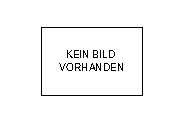
\includegraphics[width=0.7\textwidth]{images/no_pic.drawio.pdf}
    \caption{Versuchsaufbau}
    \label{fig:messaufbau}
\end{figure}


\section{Geräteliste}

\begin{itemize}
    \item 
    \item 
\end{itemize}


\section{Messwerte} \label{sec:measured-values}

\lipsum[1]

\begin{table}[h]
\begin{tabular}{ll}
Probenbezeichnung: & YYMMDD\_HHMM\_OI\_ST\_TT\_TDs \\
Beispiel: & 260218\_1445\_LiBo\_PK\_HW\_30s \\
\end{tabular}
\end{table}

\begin{longtable}{ll}
    YYMMDD & Datum der Messung \\
    HHMM & Uhrzeit der Messung \\
    OI & Operator Initials (Kürzel vom Laboranten) \\
    ST & Sample Type (Probenart): \\
     & PK: Pork \\
     & AIR: Air (Reference) \\
     & MET: Metal (Reference) \\
    TT & Treatment Type (Behandlungsart): \\
     & MR: Metal Rod (350°C) \\
     & HA: Hot Air (450°C) \\
     & CTRL: Control (unbehandelt) \\
    TDs & Treatment Duration (Behandlungsdauer in Sekunden) \\
    S01 & Sample Number (Probennummer, z.B. S01, S02...) \\
    M02 & Measurement Number (Messungsnummer an der Probe) \\
\end{longtable}

\subsection{Referenzmessungen}

\begin{longtable}{|>{\raggedright\arraybackslash}m{0.15\textwidth}|>{\centering\arraybackslash}m{0.38\textwidth}|>{\centering\arraybackslash}m{0.38\textwidth}|}
    \hline
    \textbf{Messung} & \textbf{Bild} & \textbf{Graph}  \\
    \hline
    \endhead
    \endfoot
    \label{tab:measurement-overview}
    
    Messung Metallplatte \newline $\checkmark$  &
    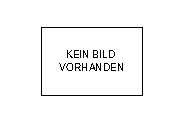
\includegraphics[width=0.25\textwidth]{images/no_pic.drawio.pdf}\newline{\textit{YYMMDD\_HHMM\_OI\_ST\_TT\_TDs}} &
    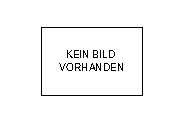
\includegraphics[width=0.25\textwidth]{images/no_pic.drawio.pdf}\newline{\textit{251222\_1015\_LiBo\_MET}} \\ \hline

    Messung Luft \newline $\checkmark$  &
    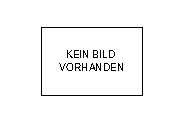
\includegraphics[width=0.25\textwidth]{images/no_pic.drawio.pdf}\newline{\textit{YYMMDD\_HHMM\_OI\_ST\_TT\_TDs}} &
    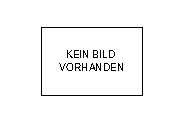
\includegraphics[width=0.25\textwidth]{images/no_pic.drawio.pdf}\newline{\textit{YYMMDD\_HHMM\_OI\_ST\_TT\_TDs}} \\ \hline

    \caption{Referenzmessungen mit Edelstahlplatte und Luft}
\end{longtable}


\subsection{Messungen von Verbrennungen durch MR}


\begin{longtable}{|>{\raggedright\arraybackslash}m{0.15\textwidth}|>{\centering\arraybackslash}m{0.38\textwidth}|>{\centering\arraybackslash}m{0.38\textwidth}|}
    \hline
    \textbf{Messung} & \textbf{Bild} & \textbf{Graph}  \\
    \hline
    \endhead
    \endfoot
    Kontrolle (0s) \newline $\checkmark$ &
    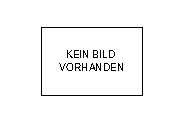
\includegraphics[width=0.25\textwidth]{images/no_pic.drawio.pdf}\newline{\texttt{YYMMDD\_HHMM\_OI\_ST\_TT\_TDs}} &
    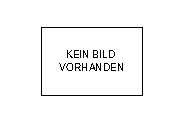
\includegraphics[width=0.25\textwidth]{images/no_pic.drawio.pdf}\newline{\texttt{YYMMDD\_HHMM\_OI\_ST\_TT\_TDs}} \\ \hline
    5s Dauer \newline $\checkmark$ &
    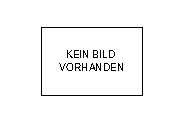
\includegraphics[width=0.25\textwidth]{images/no_pic.drawio.pdf}\newline{\texttt{YYMMDD\_HHMM\_OI\_ST\_TT\_TDs}} &
    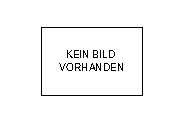
\includegraphics[width=0.25\textwidth]{images/no_pic.drawio.pdf}\newline{\texttt{YYMMDD\_HHMM\_OI\_ST\_TT\_TDs}} \\ \hline
    \caption{Messungen von Proben die mit einer Metall (350 °C) Verbrennt wurden}
\end{longtable}

\subsection{Messungen von Verbrennungen durch HA}

\begin{longtable}{|>{\raggedright\arraybackslash}m{0.15\textwidth}|>{\centering\arraybackslash}m{0.38\textwidth}|>{\centering\arraybackslash}m{0.38\textwidth}|}
    \hline
    \textbf{Messung} & \textbf{Bild} & \textbf{Graph}  \\
    \hline
    \endhead
    \endfoot

    Kontrolle (0s) \newline $\checkmark$ &
    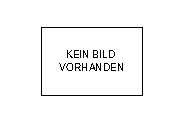
\includegraphics[width=0.25\textwidth]{images/no_pic.drawio.pdf}\newline{\texttt{YYMMDD\_HHMM\_OI\_ST\_TT\_TDs}} &
    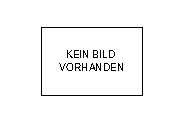
\includegraphics[width=0.25\textwidth]{images/no_pic.drawio.pdf}\newline{\texttt{YYMMDD\_HHMM\_OI\_ST\_TT\_TDs}} \\ \hline
    5s Dauer \newline $\checkmark$ &
    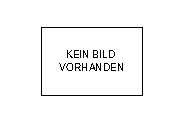
\includegraphics[width=0.25\textwidth]{images/no_pic.drawio.pdf}\newline{\texttt{YYMMDD\_HHMM\_OI\_ST\_TT\_TDs}} &
    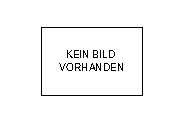
\includegraphics[width=0.25\textwidth]{images/no_pic.drawio.pdf}\newline{\texttt{YYMMDD\_HHMM\_OI\_ST\_TT\_TDs}} \\ \hline

    \caption{Messungen von Proben die mit Heißwasser (450 °C) Verbrennt wurden}
    \label{tab:measurement-overview}
\end{longtable}


\section{Äußere Bedingungen} \label{sec:external-conditions}

\lipsum[1]

\section{Besondere Beobachtungen} \label{sec:special-observations}

\lipsum[1]